%!TEX program = xelatex
%%%%%%%%%%%%%%%%%%%%%%%这是导言部分的开始%%%%%%%%

%========= 导言部分声明文档的类型=================
\documentclass{article}

	%=========导言部分可可以加载宏包=================
	\usepackage{amsmath}                % 数学公式排版宏包
	\usepackage{amssymb}                % 数学符号命令宏包
	\usepackage{amsthm}                 % 数学定理宏包
	\usepackage[UTF8]{ctex}             % 中文输入宏包
	\usepackage[a4paper]{geometry}      % 页面设置宏包
	\usepackage{setspace}               % 行间距宏包
	\usepackage{graphicx}               % 图片宏包
	\usepackage{listings}               % 代码宏包
	\usepackage{color}					% 颜色宏包
	\usepackage{xcolor}                 % 颜色处理宏包
	\usepackage{float}                  % 浮动对象式样宏包
	\usepackage{fontspec}
	
	%=========页面设置==============================
	\geometry{left=1cm,right=1cm,top=1cm,bottom=2cm}
	\onehalfspacing
	\setlength\parindent{0em}

	%=========代码格式设置============================
	\definecolor{dkgreen}{rgb}{0,0.6,0}
	\definecolor{gray}{rgb}{0.5,0.5,0.5}
	\definecolor{mauve}{rgb}{0.58,0,0.82}
	% \setmonofont{Consolas}
	\lstset{
		numbers = left, 	
		numberstyle = \color{gray}, 
		keywordstyle = \color{blue},
		commentstyle = \color{dkgreen}, 
		stringstyle = \color{mauve},
		basicstyle = \ttfamily,
		breaklines = true,
		frame = shadowbox, % 阴影效果
		rulesepcolor = \color{ red!20!green!20!blue!20} ,
		escapeinside = ``, % 英文分号中可写入中文
		xleftmargin = 2em,xrightmargin=2em, aboveskip=1em,
		framexleftmargin = 2em
	} 

%=========导言部分可以定义标题信息===============
\title{组会报告}
\author{徐益}
\date{\today}

%%%%%%%%%%%%%%%%%%%%%%%这是导言部分的结束%%%%%%%%%

%%%%%%%%%%%%%%%%%%%%%%%这是正文部分的开始%%%%%%%%%
\begin{document}
	
%=========生成标题================================
\maketitle

%=========开始正文的输入==========================

%===========第一节=================
\section{本周工作内容}

1. 实现基于DPDK传输的LTE编码调制仿真系统

2. 实现基于令牌的流量控制模块

%===========第一节=================
\section{实现基于DPDK传输的LTE编码调制仿真系统}
\begin{figure}[H]
	\centering
	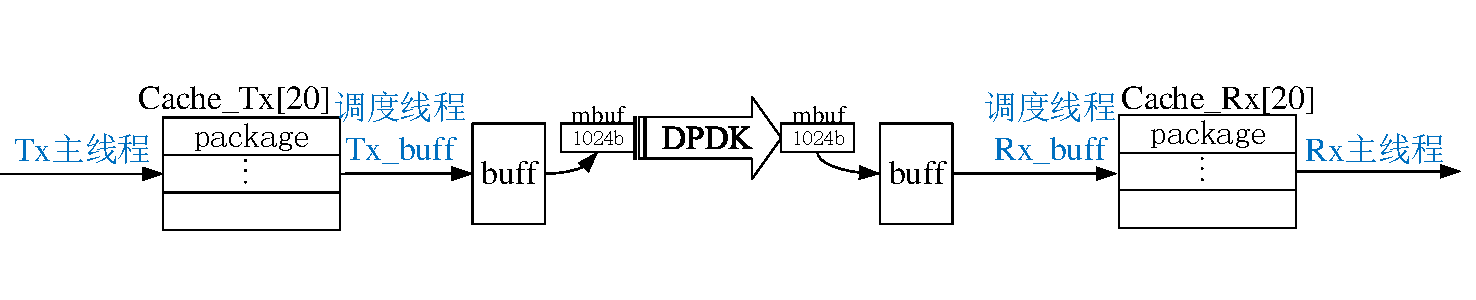
\includegraphics[width = \textwidth]{frame_sys.pdf}
	\caption{分块传输系统}
\end{figure}
\subsection{实现过程中的问题}
1. 无法接收部分包
\begin{figure}[H]
	\centering
	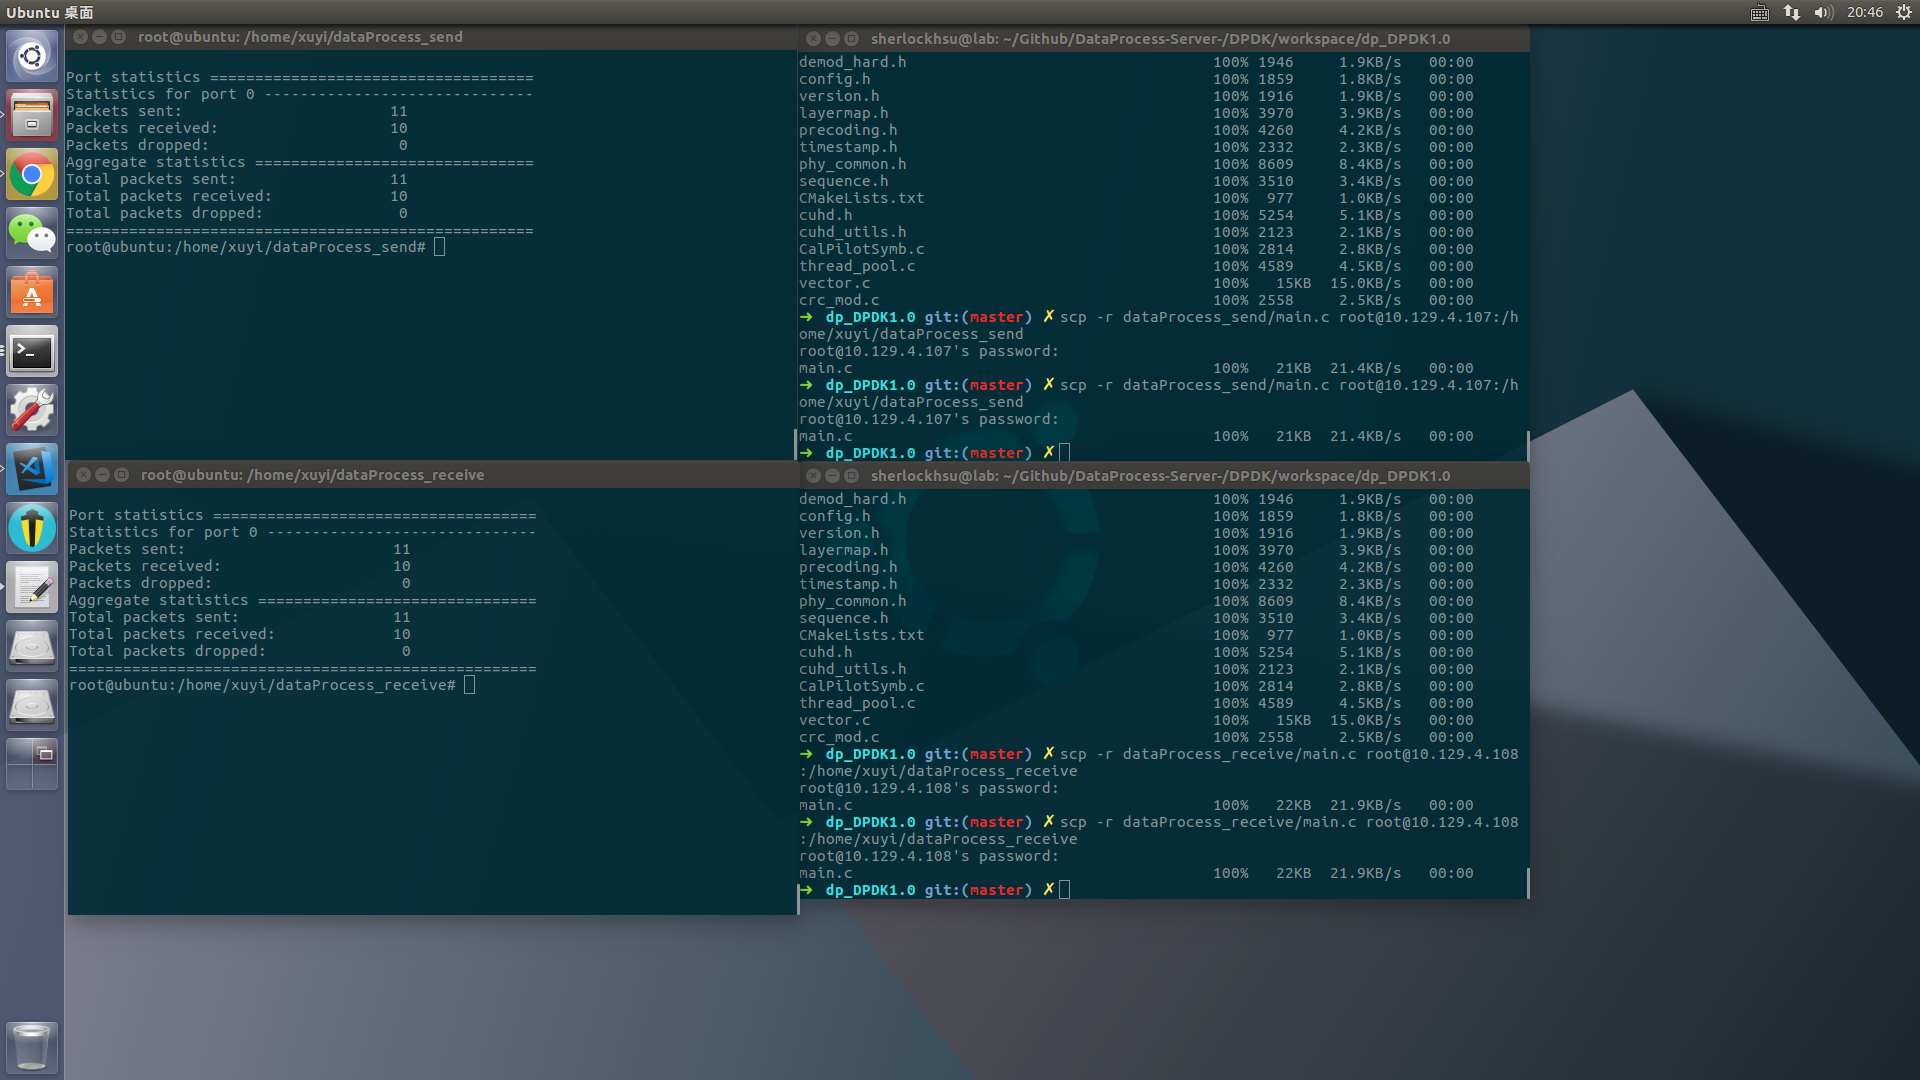
\includegraphics[width = .8\textwidth]{result_drop.png}
	\caption{无法接收部分包}
\end{figure}
\begin{figure}[H]
	\centering
	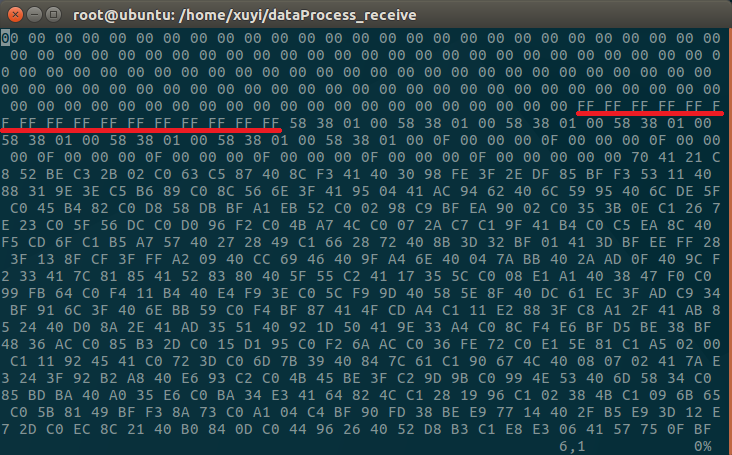
\includegraphics[width = .8\textwidth]{drop_fix.png}
	\caption{添加全1位}
\end{figure}
2. 接收端速率匹配错误
\begin{figure}[H]
	\centering
	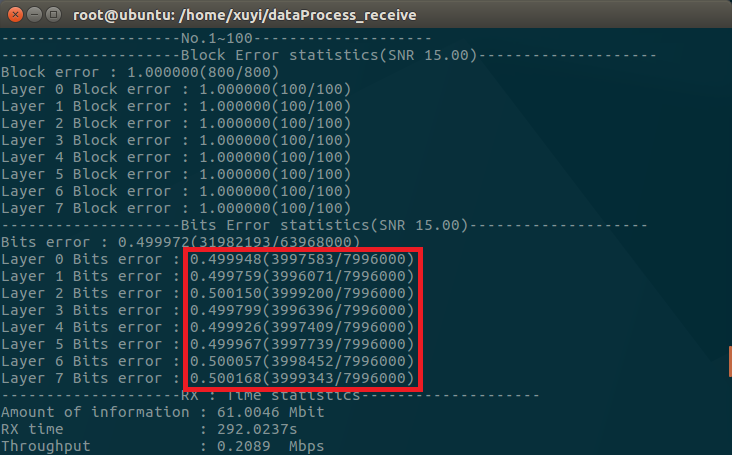
\includegraphics[width = .8\textwidth]{receive_res_ber.png}
	\caption{接收端服务器显示}
\end{figure}
\begin{figure}[H]
	\centering
	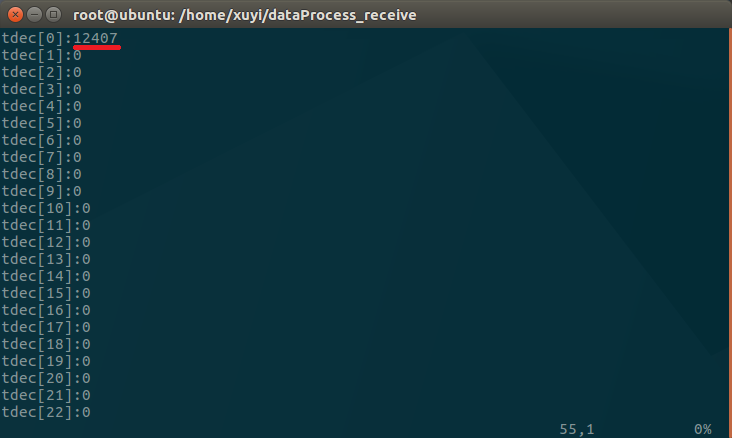
\includegraphics[width = .6\textwidth]{tdec_error.png}
	\caption{速率匹配错误}
\end{figure}
\begin{lstlisting}
void srslte_rm_turbo_gentables();
\end{lstlisting}
\subsection{实现结果}
\begin{figure}[H]
	\centering
	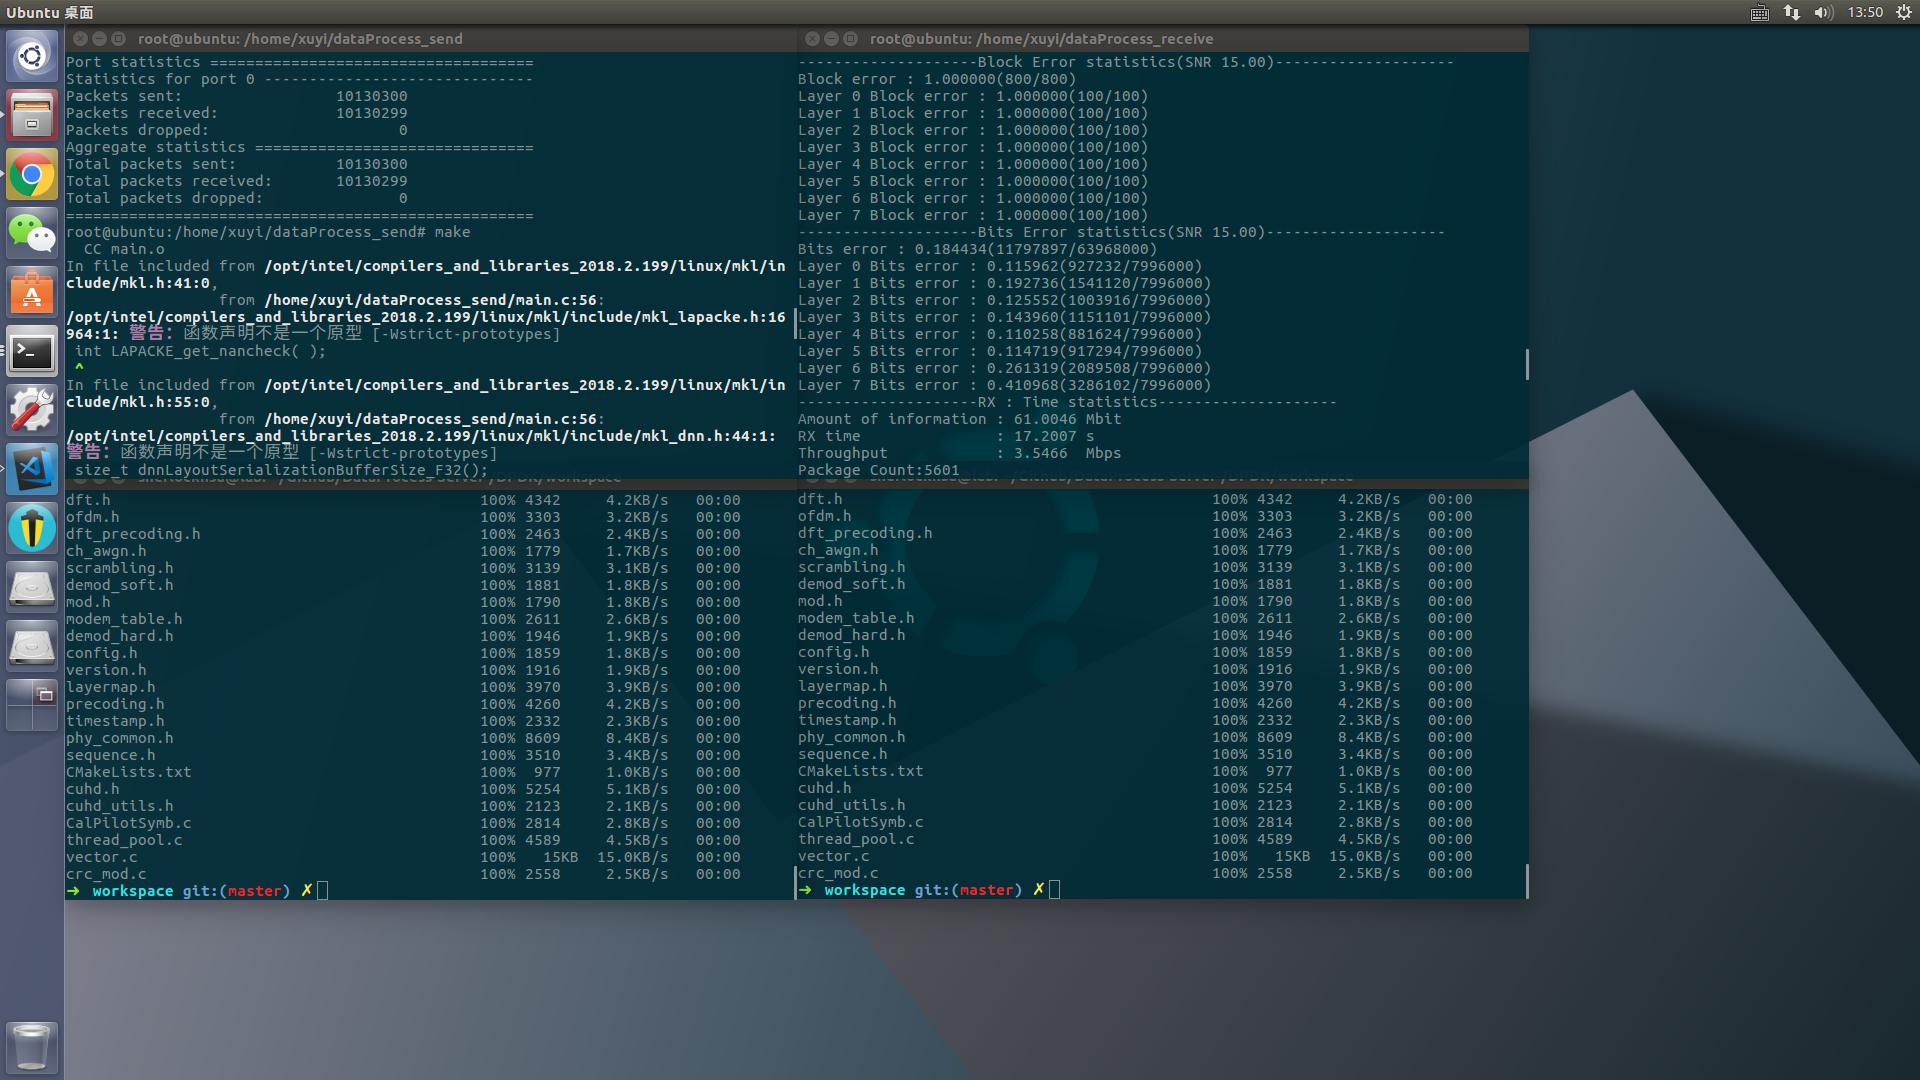
\includegraphics[width = .6\textwidth]{result1.png}
	\caption{接收端服务器显示}
\end{figure}

%===========第二节=================
\section{实现基于令牌的流量控制模块}
\begin{figure}[H]
	\centering
	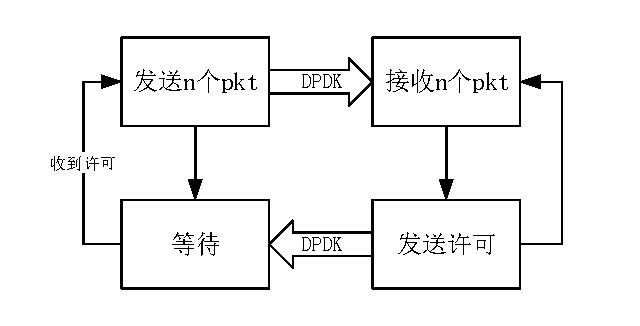
\includegraphics[width = .6\textwidth]{flow_traffic.pdf}
	\caption{原流量控制系统}
\end{figure}
\begin{figure}[H]
	\centering
	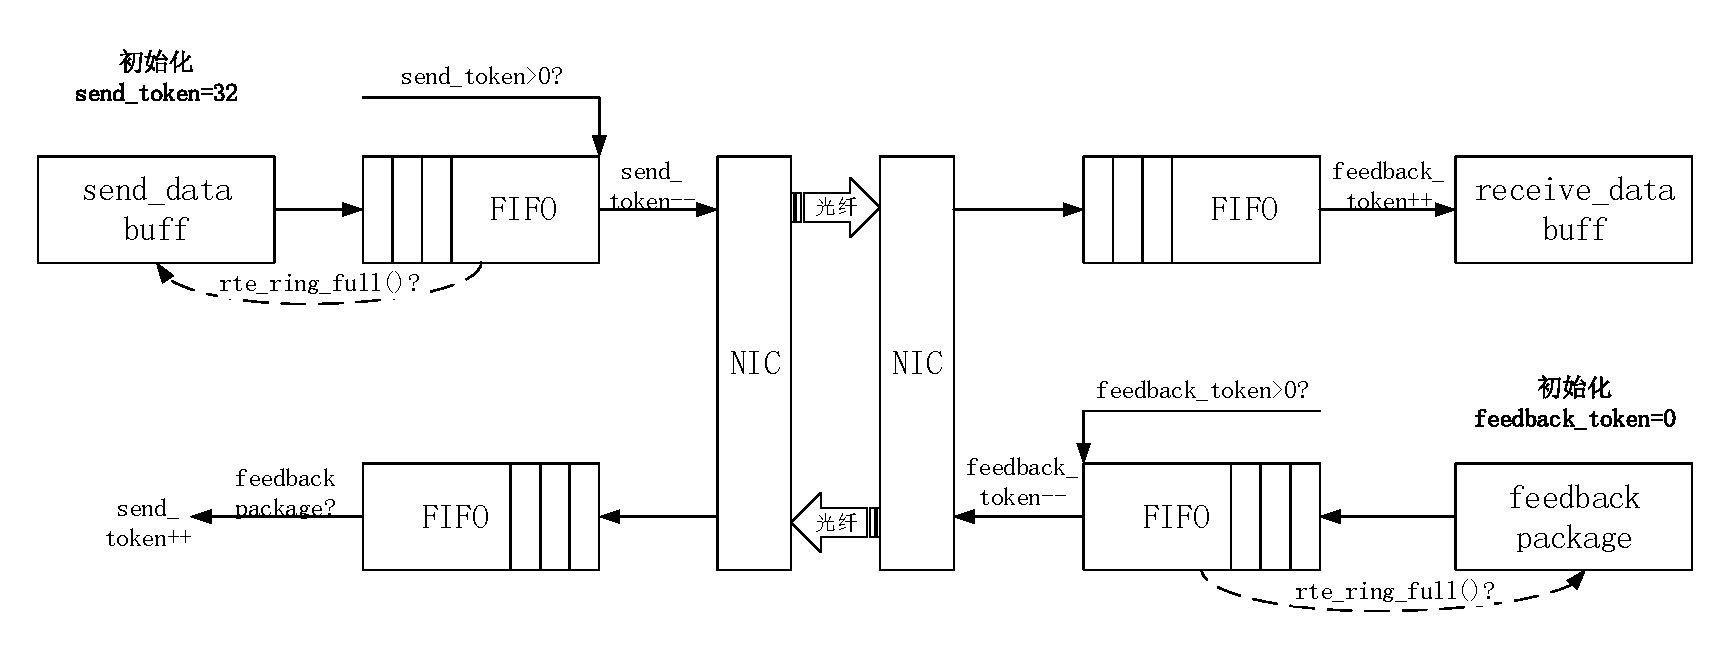
\includegraphics[width = \textwidth]{frame_token.pdf}
	\caption{基于令牌的流量控制系统}
\end{figure}

%===========第三节=================
\newpage
\section{仍存在的问题}
1. 内存溢出错误
\begin{figure}[H]
	\centering
	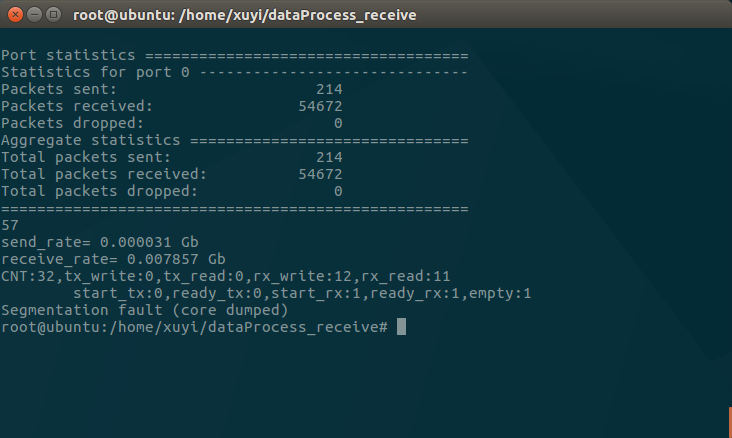
\includegraphics[width = .8\textwidth]{receive_res_dumped.png}
	\caption{内存溢出报错}
\end{figure}
2. 拷贝过程的简化
\begin{figure}[H]
	\centering
	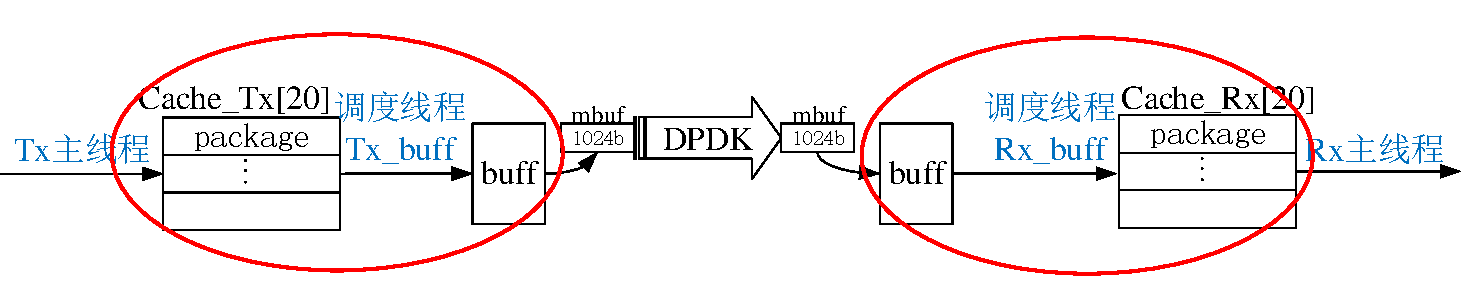
\includegraphics[width = \textwidth]{frame_sys_copy.pdf}
	\caption{分块传输系统}
\end{figure}

%===========第四节=================
% \section{其他改进方向}
% 1. 选择更大的DPDK发送页。\\

% 2. 选择更优的流量控制策略。\\

%===========下周计划=================
\section{下周计划}
1. 解决内存溢出错误

2. 实现拷贝过程的简化

3. 期末复习

\end{document}
%%%%%%%%%%%%%%%%%%%%%%%这是正文部分的结束%%%%%%%%%%%%